Il transistore MOSFET (\emph{Metal-Oxide Semiconductor Field-Effect Transistor}) è un dispositivo elettronico utilizzato sia in circuiti digitali, in cui è impiegato principalmente come interruttore controllato in tensione, sia in circuiti analogici, in cui è impiegato come amplificatore di segnale o come resistenza controllata in tensione.\\

\begin{figure}[H]
  \centering
  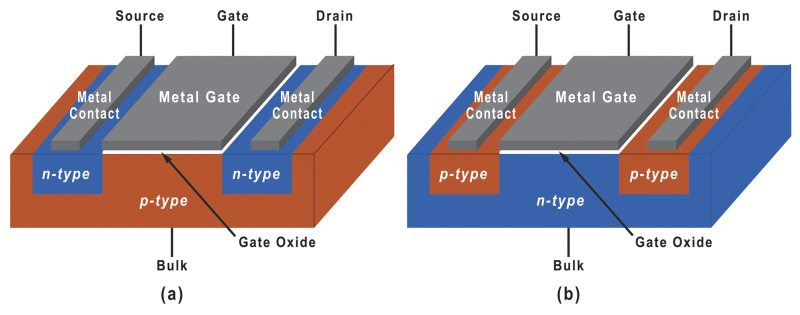
\includegraphics[width=0.80\textwidth]{./capitolo1/MOSFET/StrutturaMosfet}
  \caption[Struttura dei MOSFET]{MOSFET a canale N (a) e a canale P (b) \cite{transistore_MOSFET:From_MOSFET_to_FinFET_to_GAAFET}}
  \label{fig:StrutturaMosfet}
\end{figure}

Come mostrato nella figura \ref{fig:StrutturaMosfet}, i MOSFET sono caratterizzati da quattro terminali: \emph{source} (S), \emph{drain} (D), \emph{gate} (G) e \emph{bulk} (B).
Il MOSFET a canale N viene realizzato su un substrato di tipo P in cui sono innestate due regioni fortemente drogate di tipo N. Queste due regioni presentano delle metallizzazioni che formano i terminali di \emph{source} e di Drain. Sul substrato, tra le due regioni fortemente drogate, è presente un sottile strato di ossido che fa da isolante (storicamente $SiO_2$, attualmente si usano anche altri ossidi) sopra il quale si trova una metallizzazione che forma il contatto di Gate. Il \emph{bulk} (o substrato), solitamente cortocircuitato con il Source, deve essere connesso al potenziale più basso (massa) negli NMOS e al potenziale più alto presente nel circuito (alimentazione positiva) nei PMOS. \\

\subsection{Regioni di funzionamento e caratteristica $I-V$}


In un MOSFET a canale N, in linea generale, può scorrere una corrente $I_D$ che va dal \emph{drain} al \emph{source} in funzione di due tensioni (sempre non negative): 
\begin{itemize}
  \item la tensione presente tra \emph{drain} e \emph{source} ($V_{DS}$);
  \item la tensione presente tra \emph{gate} e \emph{source} ($V_{GS}$).  
\end{itemize}

La dipendenza di $I_D$ da tali tensioni è messa in evidenza dalla caratteristica corrente-tensione (figura \ref{fig:caratteristica-I-V}).

\begin{figure}[h]
  \centering
  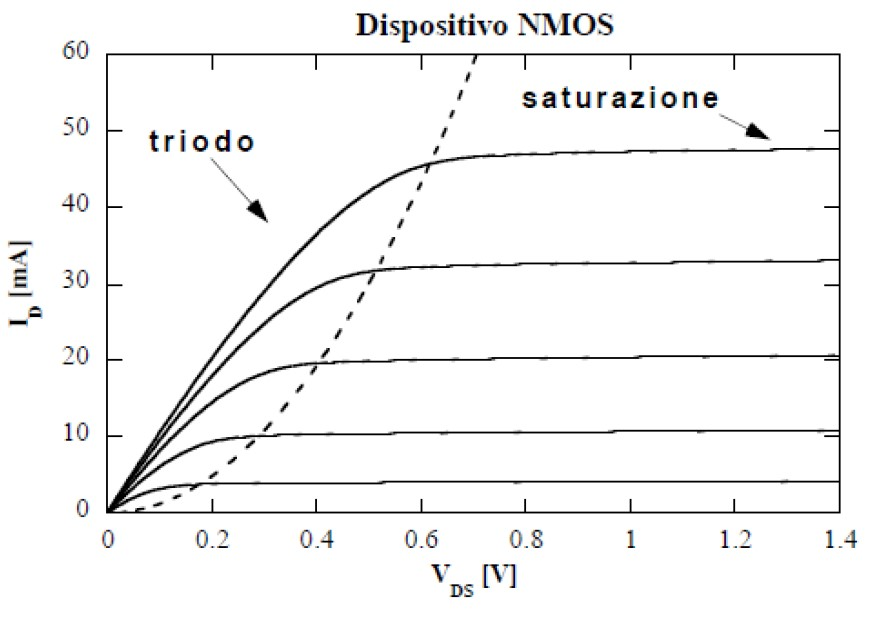
\includegraphics[width=0.80\textwidth]{./capitolo1/MOSFET/Caratteristica-I-V}
  \caption[Caratteristica $I-V$ di un MOSFET a canale N]{Caratteristica $I-V$ di un MOSFET a canale N}
  \label{fig:caratteristica-I-V}
\end{figure}

Quando $V_{GS} = 0$, indipendentemente dal valore di $V_{DS}$, la corrente $I_D$ è nulla, poiché la giunzione P-N composta da substrato e \emph{drain} e quella formata da substrato e \emph{source} sono in regione inversa. \\
Aumentando il valore di $V_{GS}$, le lacune presenti nel substrato si allontanano dalla regione direttamente al di sotto dell'ossido, creando una
zona svuotata di portatori di carica liberi. Gli elettroni presenti nel semiconduttore
vengono attirati, creando una regione di canale di tipo N che unisce il
Source e il Drain. Questo canale permette il passaggio di corrente, ma per crearlo è necessario che $V_{GS}$ abbia un valore almeno pari alla cosiddetta tensione di soglia ($V_{th}$). Finché $V_{GS} < V_{th}$, il MOSFET si trova in regione di \emph{cutoff} e $I_D \simeq 0$.

Nel momento in cui $V_{GS}$ eguaglia e supera $V_{th}$, il canale di conduzione è completo e inizia a scorrere corrente, seguendo leggi matematiche differenti in funzione del valore di $V_{DS}$.

\vspace*{0.5cm}

Se $V_{DS} < V_{GS} -  V_{th}$, il MOSFET è in regione lineare o di triodo e la corrente di \emph{drain} segue la seguente legge:\\

\begin{equation}
  I_D = 2k_n\left[ \left(V_{GS}-V_{th}\right)V_{DS} - \frac{{V_{DS}}^2}{2}\right]
\end{equation}

dove:

\begin{align*}
   k_n &= \frac{1}{2}\mu_n C_{ox}\frac{W}{L} \\
   \mu_n &= \text{mobilità degli elettroni} \\
   C_{ox} &= \text{capacità dell'ossido} \\
   W &= \text{larghezza del canale} \\
   L &= \text{lunghezza del canale}
\end{align*}

Se, invece, $V_{DS} > V_{GS} -  V_{th}$ il MOSFET si trova in regione di saturazione e la corrente di \emph{drain} ha un andamento che segue la legge:\\
\begin{equation}
  I_D = k_n\left(V_{GS}-V_{th}\right)^2 (1+\lambda V_{DS})
\end{equation}
dove $\lambda$ è un parametro che tiene conto della modulazione della lunghezza di canale introdotta dalla tensione $V_{DS}$.\\

Tutto quanto detto finora sui MOSFET a canale N vale in maniera analoga per i MOSFET a canale P.
Altri parametri verranno descritti nel prossimo capitolo.

\subsection{Modello per piccolo segnale e sorgenti di rumore}
Il modello per piccolo segnale rappresenta il funzionamento del MOSFET nel momento in cui si fissa il punto di lavoro in continua e si fornisce in ingresso al dispositivo un segnale con un'ampiezza sufficientemente piccola da non alterarne il funzionamento. \\

In prima approssimazione, il MOSFET si comporta come un generatore di corrente controllato in tensione che emette una corrente proporzionale al valore di $V_{GS}$. La costante di proporzionalità è la transconduttanza di canale $g_m$, che dipende dal punto di lavoro ed è descritta meglio al paragrafo \ref{sec:transconduttanza}. Un modello più accurato prevede che, quando il MOSFET è in saturazione, la corrente di \emph{drain} dipenda anche da $V_{DS}$ in modo lineare. Nel circuito equivalente per piccolo segnale, perciò, in parallelo al generatore di corrente, è presente una resistenza $r_0 = \frac{1}{\lambda I_{D,sat}}$ che viene attraversata da una corrente prodotta dalla differenza di tensione tra \emph{drain} e \emph{source} e che va a sommarsi a quella generata dal generatore ideale, figura \ref{fig:piccolo_segnale}.

\begin{figure}[t]
  
  \centering
  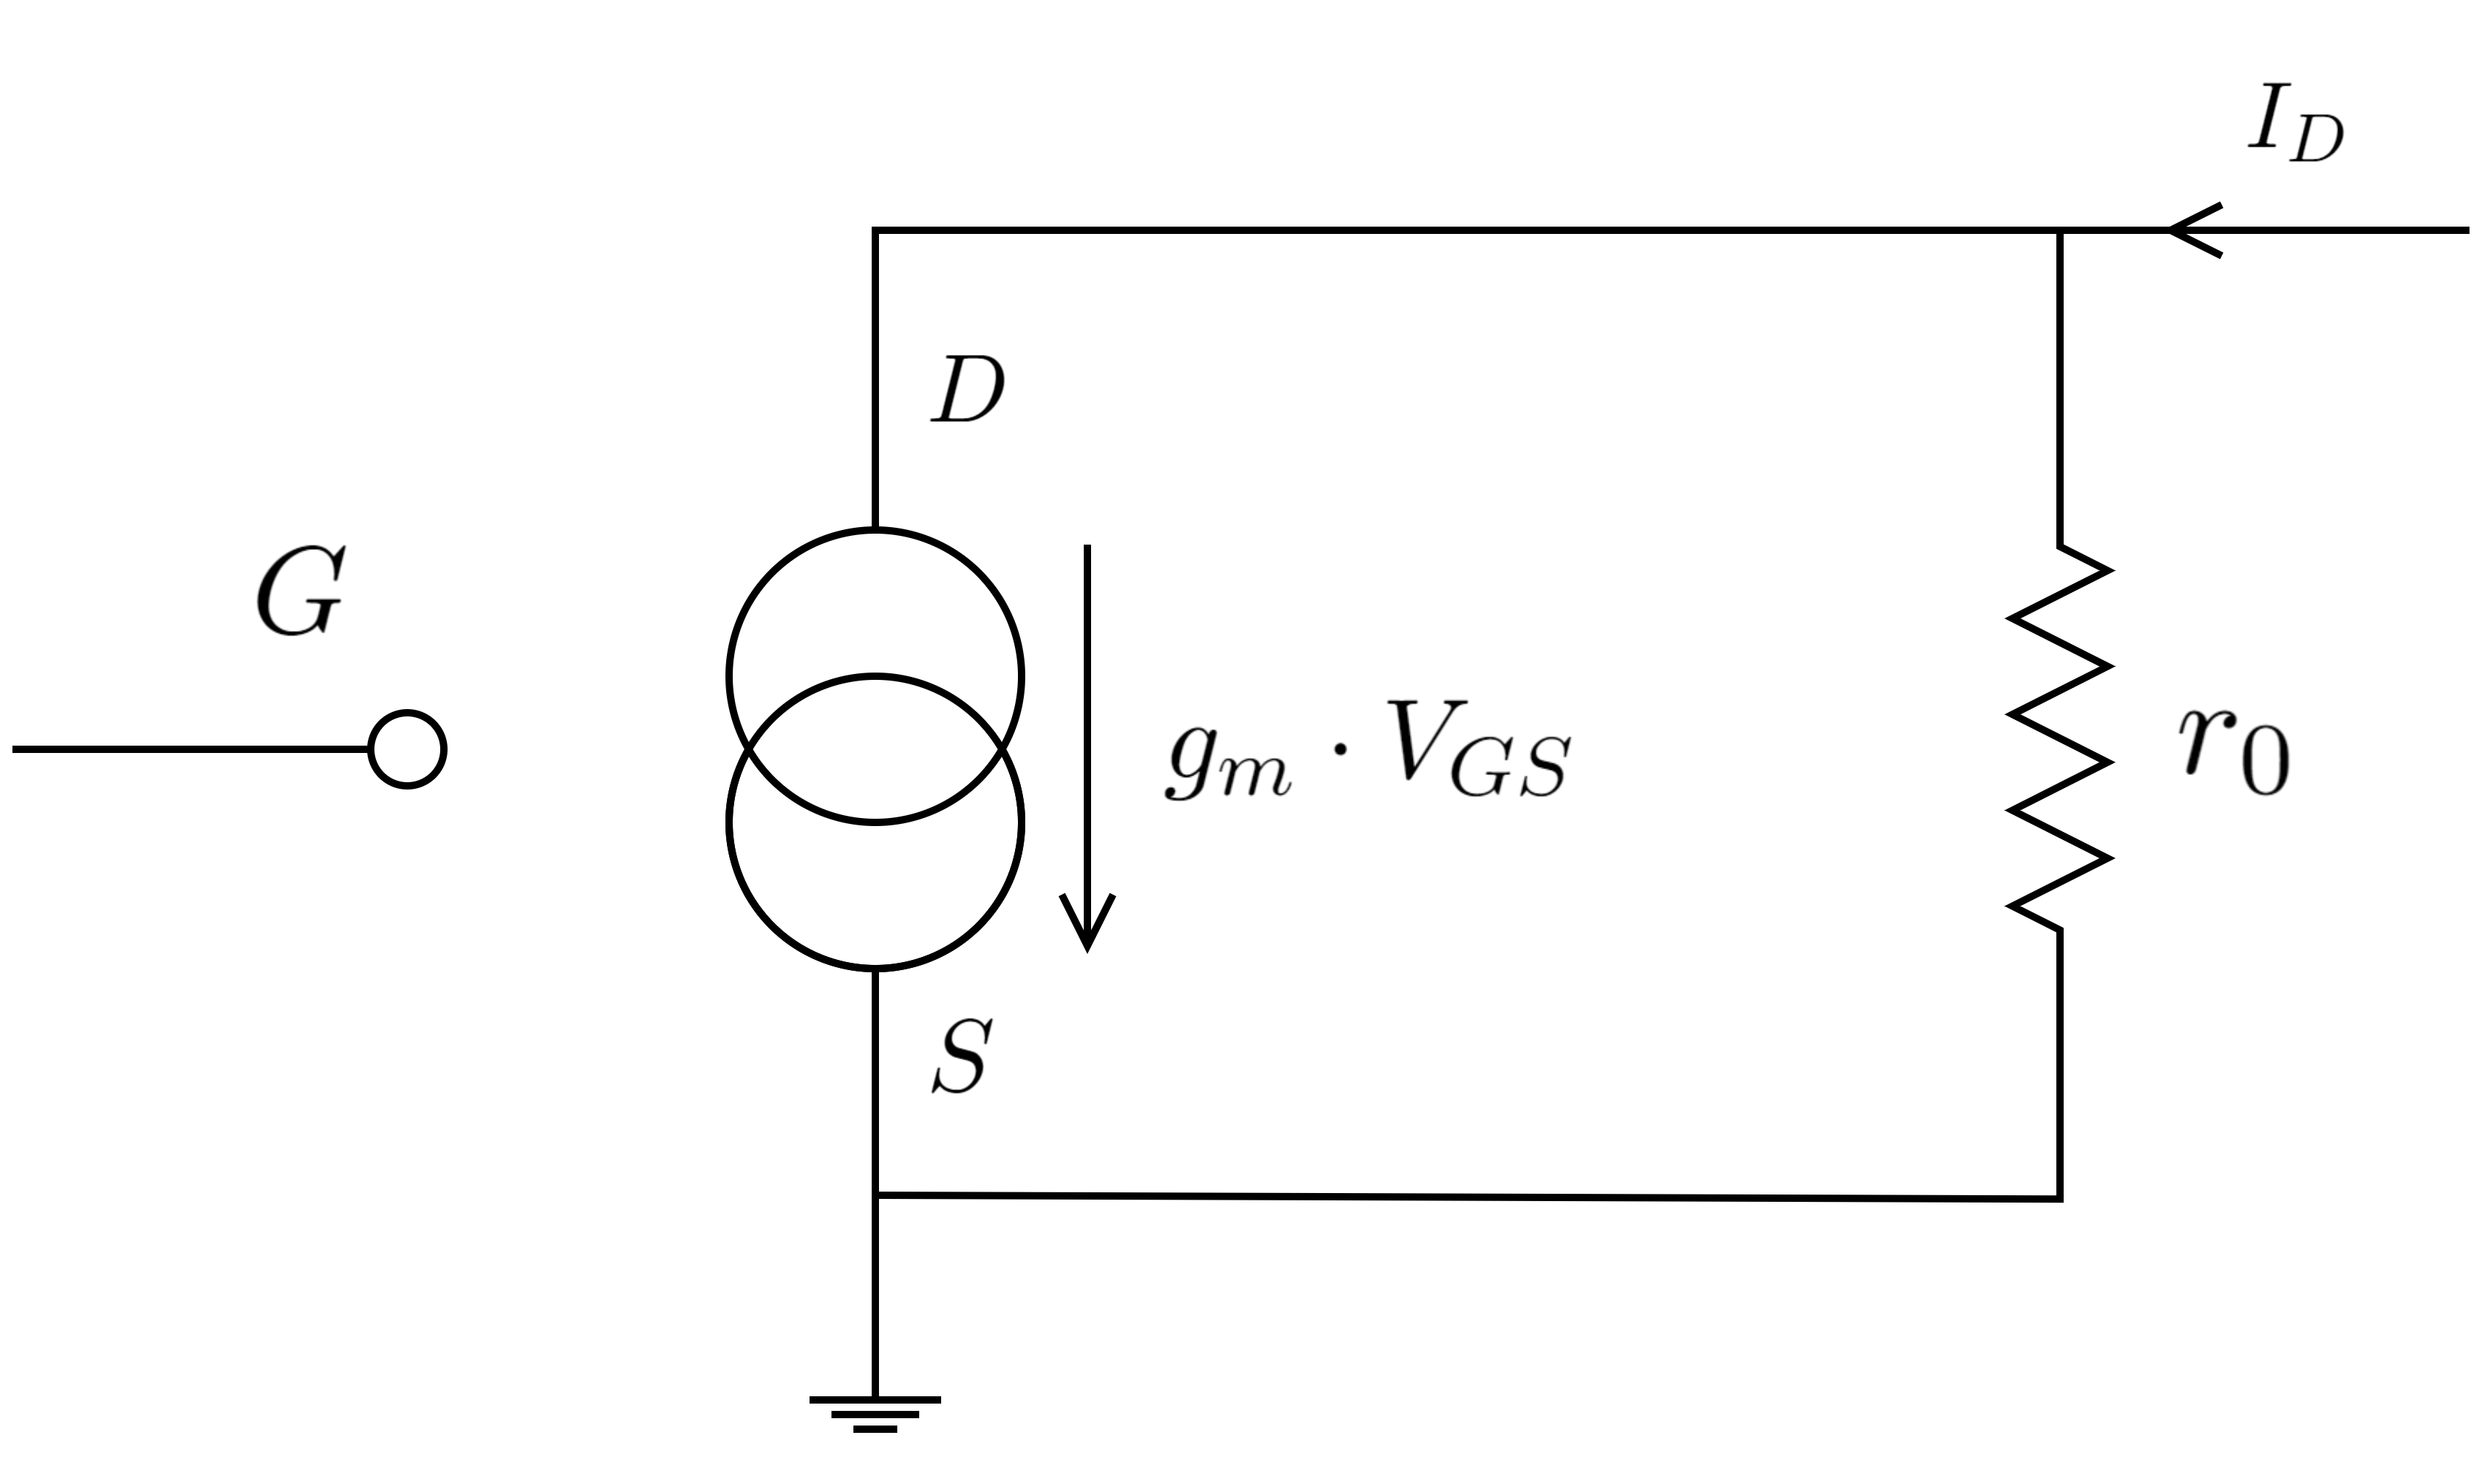
\includegraphics[width = 0.55\linewidth]{./capitolo1/MOSFET/PiccoloSegnale/PiccoloSegnale.png}
  \caption[Modello piccolo segnale]{Modello piccolo segnale}
  \label{fig:piccolo_segnale}

\end{figure}

\vspace*{0.5cm}

Per comprendere al meglio l'effettivo comportamento dei MOSFET, però, bisogna considerare che il segnale in uscita al MOSFET subisce delle interferenze dovute al rumore generato all'interno del dispositivo stesso. Esistono diverse sorgenti di rumore; qui di seguito si descrivono le principali.

\paragraph*{Rumore termico di canale o rumore bianco}
Il canale di un dispositivo è composto da materiale resistivo e quindi è sorgente di rumore termico. Tale sorgente può essere rappresentata come un generatore di tensione la cui densità spettrale di potenza segue leggi differenti in base alla lunghezza del canale $L$.  Infatti, se tale dimensione è nell'ordine delle frazioni di micron, subentrano i cosiddetti effetti di canale corto, che comportano l'aumento del rumore e che non possono essere ignorati.
Poiché tutti i dispositivi presi in considerazione ricadono in questa categoria, la trattazione del rumore termico di canale si concentra sulla descrizione della legge matematica legata ai dispositivi a canale corto, ovvero:

\begin{equation}
  S_w = 4 K_B T \frac{\alpha_w n_{sub} \gamma}{g_m}
\end{equation}
Dove $K_B$ è la costante di Boltzmann e T è la temperatura assoluta. $\alpha_w$ è il fattore di rumore in eccesso che tiene conto degli effetti di canale corto. Analisi approfondite (non mostrate in questa tesi) mostrano che per i dispositivi analizzati questo fattore ha valore 1, tranne per gli NMOS con lunghezza di canale $L = 30mn$, per i quali $\alpha_w > 1$. $n_{sub}$ è un coefficiente proporzionale al reciproco della pendenza della caratteristica $I_D-V_{GS}$ nella regione di sotto-soglia. $\gamma$ è il coefficiente di rumore termico di canale che, per i dispositivi nanometrici, può essere espresso come:

\begin{equation}
  \gamma = \frac{1}{1 +  \frac {I_D L}{{I_Z}^* W}}\left(\frac{1}{2} + \frac{ 2 I_D L}{3 {I_Z}^* W}\right)
\end{equation}

dove ${I_Z}^*$ è la corrente di \emph{drain} caratteristica normalizzata, che si può estrarre dalle misure statiche.

Il rumore termico di canale può essere anche espresso sotto forma di resistenza equivalente $R_{eq}$, tramite l'equazione:

\begin{equation}
  R_{eq} = \frac{S_w}{4 K_B T} = \alpha_w \frac{n_{sub} \gamma}{g_m}
\end{equation}

\paragraph*{Flicker Noise}
A basse frequenze, prevale una componente di rumore del tipo $1/f$, la cui densità spettrale è inversamente proporzionale alla frequenza del segnale:

\begin{equation}
  S_{\frac{1}{f}} \left(f\right) = \frac{K_f}{C_{ox}^2 W L} \frac{1}{f^{\alpha_f}}
\end{equation}
dove $K_f$ è un parametro che dipende dalla tecnologia e $\alpha_f$ tiene conto della dipendenza dalla frequenza.
Il rumore $\sfrac{1}{f}$ è causato da una variazione della densità di portatori dovuto a fluttuazioni del potenziale superficiale; i portatori, all'interfaccia tra ossido e canale, vengono intrappolati e successivamente rilasciati e questo ha un effetto più evidente alle frequenze più basse

In passato, a parità di tecnologia, polarizzazione e dimensioni, il flicker noise è minore nei MOSFET a canale P, rispetto a quelli a canale N. Infine, il processo di \emph{scaling} dei dispositivi influenza la quantità di questo tipo di rumore: analizzando l'equazione della densità spettrale, si nota come la riduzione delle dimensioni del canale comportano un aumento di rumore. Al contrario, la diminuzione dello spessore del \emph{gate} porta all'aumento della sua capacità e quindi ad una riduzione del rumore. Allo stesso tempo, però, un \emph{gate} più sottile potrebbe presentare altre problematiche, quindi il fattore $K_f$ potrebbe non diminuire come aspettato e necessita per tanto un costante monitoraggio. 

\paragraph*{Rumore associato alla corrente di Gate}
Fino ad ora si è considerata solo la corrente $I_D$ che va da dal \emph{drain} al \emph{source} (o viceversa, in base al tipo di canale). In realtà esiste anche una corrente $I_G$ che attraversa il Gate, che in generale, appunto, è trascurabile, se confrontata con  $I_D$. Infatti l'ossido presente tra il contatto di \emph{gate} e il substrato fa da barriera di potenziale all'iniezione dei portatori di carica. Questa barriera può essere comunque attraversata dai portatori con temperatura (e quindi energia cinetica) maggiore. Con la riduzione dello spessore del gate, l'energia necessaria per iniettare i portatori attraverso il \emph{gate} diminuisce e quindi $I_G$ diventa meno trascurabile.

\paragraph*{Altre sorgenti di rumore}
Ci sono infine sorgenti di rumore legate alla presenza di resistenze parassite nel Gate, nel Substrato e tra \emph{drain} e Source.